%==============================================================================
% Journal extension of the SBR/LARS 2026 paper (#34344).
% Target: Digital Engineering (Elsevier), Special Issue VSI:DTE_DigiTwin2026.
% Class: elsarticle, numeric references (elsarticle-num).
%
% Skeleton of 23/09/2026 (lote 1 do chat do artigo). Mapa secao -> artefato ->
% numero -> figura em docs/journal/MAPEAMENTO_ARTIGO.md. Tabelas em tables/ e
% figuras em figures/ sao geradas pelos modulos do dtssl a partir dos artefatos
% de results/ (nao editar a mao):
%   dtssl analysis run journal_tables
%   dtssl fig fig_journal_identifiability | fig_journal_league_sims | fig_journal_closed_loop
% Regras: nenhum numero fora de results/CHANGELOG.md ou de um artefato citado;
% nenhuma referencia fora de refs/references.bib (copia de latex/refs) ou da
% lista de incluidos da SLR; nenhum paragrafo copiado do artigo do SBR; sem
% travessao. \pending{} e REPLACE-ME tem de sumir antes da submissao.
%
% Build: latexmk -pdf main.tex   (ou pdflatex, bibtex, pdflatex, pdflatex)
%==============================================================================
\documentclass[preprint,12pt]{elsarticle}
% Submission: \documentclass[review,12pt]{elsarticle} (double spacing) + line numbers.
\usepackage{amsmath,amssymb}
\usepackage{graphicx}
\usepackage{booktabs}
\usepackage{adjustbox}
\usepackage{siunitx}
\usepackage{xcolor}
\usepackage[hidelinks]{hyperref}
\usepackage{lineno}
\graphicspath{{figures/}}

% --- notation (same symbols as the SBR paper) --------------------------------
\newcommand{\epos}{e_{\mathrm{pos}}}
\newcommand{\eang}{e_{\mathrm{ang}}}
\newcommand{\SEtwo}{\mathrm{SE}(2)}
\newcommand{\Td}{T_{d}}
\newcommand{\hRef}{h_{\mathrm{ref}}}

% --- drafting marker: must be absent at submission ------------------------------
\newcommand{\pending}[1]{\textcolor{gray}{\emph{[Pending: #1]}}}

\journal{Digital Engineering}

\begin{document}

\begin{frontmatter}

% Working title (plan, option 1). Option 2: "What operational logs can identify:
% excitation regime, cross-coupling and fair baselines in a behavioral digital twin
% of an omnidirectional robot". Decide with the advisor.
\title{Identifiability-aware behavioral digital twins from operational data: a validated grey-box plant for an omnidirectional robot with physics-based and league-simulator baselines}

% Authors and affiliations: REPLACE-ME (decide authorship with the advisor).
\author[cin]{REPLACE-ME}
\affiliation[cin]{organization={Centro de Informática, Universidade Federal de Pernambuco},
            city={Recife},
            country={Brazil}}

\begin{abstract}
\pending{abstract, 200 to 250 words, written last (WP4).}
\end{abstract}

\begin{keyword}
digital twin \sep system identification \sep identifiability \sep grey-box modeling \sep validation \sep omnidirectional robot
\end{keyword}

\end{frontmatter}

\linenumbers

%==============================================================================
% 1 INTRODUCTION
% Plano: reality gap nas plataformas de futebol de robos e, em geral, nos gemeos de
% robos moveis; a camada de planta de um gemeo (mapa comando -> movimento); dados
% operacionais que a equipe ja grava; a pergunta (o que esses dados identificam e o
% que nao identificam); seis contribuicoes; o artigo do SBR como versao preliminar.
% Fonte: SBR sec. I (reescrever, nao copiar); plano §2 (tese); refs de references.bib.
% Contribuicoes candidatas (fechar com a orientadora):
%  (1) identificabilidade como propriedade do regime e da realimentacao (C1, C1b, r3);
%  (2) mecanismo do vies do yaw: acoplamento translacao -> guinada (C1b + MIMO/WP2);
%  (3) regra de triagem antes do ajuste (excitation_per_dof, analyze_omega_excitation);
%  (4) protocolo de fidelidade observacional pre-registrado, agnostico ao simulador,
%      com condicao inicial justa (harness, C2b, C2b2);
%  (5) comparacao com fisica e simuladores da liga sob o mesmo protocolo (C2a, C2b, C2b2);
%  (6) plausibilidade em malha fechada (C4, B3).
% Obrigatorio: "A preliminary version of this work appeared in \cite{sbr2026preliminary};
% this article adds ...".
%==============================================================================
\section{Introduction}
\label{sec:intro}

\pending{motivation, question, contributions, relation to the preliminary version \cite{sbr2026preliminary}.}

%==============================================================================
% 2 RELATED WORK
% Plano: gemeos de robos moveis (construcao e validacao); identificacao grey-box
% para gemeos; identificacao em malha fechada; calibracao sim-to-real a partir de
% dados; simuladores da liga (grSim, ER-Force) e RL em SSL.
% Fontes: SBR sec. II + backlog JINT item F + SLR (so a lista de incluidos que o
% Victor trouxer; RQ1 e RQ2). Referencias ja verificadas: refs/references.bib.
% ER-Force: nao ha entrada no .bib; citar o simulador exige uma fonte verificada
% (repositorio/artigo) trazida pelo Victor ou pela SLR.
%==============================================================================
\section{Related work}
\label{sec:related}

\subsection{Digital twins of mobile robots}
\pending{construction and validation of mobile-robot twins; what fidelity they report.}

\subsection{Grey-box and closed-loop identification}
\pending{grey-box identification for twins; identifiability under feedback \cite{gustavsson1977identification,vandenhof1998closedloop,forssell1999closedloop}.}

\subsection{Simulators of the league and sim-to-real calibration}
\pending{grSim \cite{monajjemi2012grsim}, rSim/rSoccer \cite{martins2021rsoccer}, ER-Force (reference to be verified), calibration from data \cite{tiboni2023dropo}.}

%==============================================================================
% 3 ROBOT, DATA AND INSTRUMENTATION
% Plano: o robo (4 rodas omni, 60/135/225/300 graus, R e r do CAD), firmware (PI por
% roda, zona morta por roda 1.567 rad/s), visao SSL a 60 Hz, logs de competicao (46
% eventos, 4 rotulos, hold-out congelado de 10), coleta dedicada de rotacao (escada),
% sessao gravada da estrategia contra o gemeo (B3); cadeia de medicao (figura do
% camera-ready com fotos).
% Fontes: config/robot_geometry.json, config/holdout_events.json, CHANGELOG 2026-07-24
% (D9, rotate), session_report_sessao_01_20260907_2059 (B3).
%==============================================================================
\section{Robot, data and instrumentation}
\label{sec:data}

\pending{robot and firmware; competition logs and the frozen hold-out; the dedicated rotation collection; the recorded closed-loop session; measurement chain (adapt the camera-ready figure).}

%==============================================================================
% 4 MODELS
% Plano: planta FOPDT por DOF (Eq. do SBR); modelo acoplado de primeira ordem (Eq. do
% modulo coupled_mimo_check: y_i[k] = A_i y_i[k-1] + sum_j B_ij u_j[k-1-M_ij]);
% discretizacao e alinhamento (convencao da planta); estimadores (P1D por erro de
% predicao no MATLAB para o theta promovido; minimos quadrados separaveis em erro de
% saida para a checagem MIMO); regra de triagem pre-ajuste (fracao de atuacao por
% comando e variancia explicada: 96/94/56 %).
% Fontes: config/twin_params.json; docs/PREREGISTRO_MIMO_CHECK_20260923.md;
% results/excitation_per_dof_20260810_1022.md; results/omega_excitation_analysis_20260807_133917.json.
%==============================================================================
\section{Models and estimators}
\label{sec:models}

\pending{per-DOF FOPDT plant; coupled first-order model; discretization; estimators; pre-fit screening rule.}

%==============================================================================
% 5 VALIDATION PROTOCOL
% Plano: harness free-run (janelas re-ancoradas em SE(2), stride 15, H_max 90,
% horizontes 0.1 a 1.5 s, h_ref 0.4 s), bins de movimento, gate pre-registrado e
% unidade por evento; replay via ssl-simulation-protocol (teleporte, relogio de
% parede, ancora da visao, tau0) e a pre-rolagem; criterios de validade do
% instrumento (V e V'); pre-registros e desvios declarados (C1b v1 e C4 mantidos).
% O harness e o servidor aparecem como METODO, nao como contribuicao de plataforma.
% Fontes: config/metrics.json; docs/PREREGISTRO_C2B_SIMULADORES_LIGA_20260910.md;
% docs/PREREGISTRO_C2B2_PREROLAGEM_20260916.md; demais PREREGISTRO_*.md.
%==============================================================================
\section{Validation protocol}
\label{sec:protocol}

\pending{free-run harness and metric; statistics by event; protocol replay with pre-roll; instrument validity; pre-registration and declared deviations.}

%==============================================================================
% 6 RESULTS I: IDENTIFIABILITY BY EXCITATION REGIME
% Plano: modelo identificado (Tab.) e o ajuste de yaw em malha fechada (K 1.378, fit
% 44.8 %); diluicao (1 % da atuacao por roda, 56 % da variancia); C1 (gerador linear
% recupera theta* sempre que ha excitacao; fit % mede SNR); C1b (gerador fisico
% reproduz a inflacao +16.5 / +27.4 %, controle sem translacao 0.988 / 0.930,
% rotacao dedicada 0.996): Fig. e Tab.
% Fontes: tab_journal_identified, tab_journal_insilico_yaw, fig_journal_identifiability
% (geradas); CHANGELOG 2026-09-07 15:52 (C1) e 20:45 (C1b v2).
%==============================================================================
\section{Results I: identifiability follows the excitation regime}
\label{sec:res-ident}

% ==============================================================================
% tab_journal_identified: generated by `dtssl analysis run journal_tables` (dtssl.analysis.journal_tables).
% Do not edit by hand: re-run the generator. Sources:
%   config/twin_params.json (K, tau, Td)
%   results/CHANGELOG.md 2026-06-14 10:24 and 2026-07-24 17:35 (hold-out fits)
%   results/loo_translational_20260810_1743.md
%   results/r3_closedloop_omega_fit_20260810_1036.md
% ==============================================================================
% Needs \usepackage{booktabs,adjustbox}.
\begin{table*}[t]
\centering
\caption{Identified per-DOF first-order-plus-dead-time parameters and hold-out fit (Eq. fit). The yaw channel fitted on closed-loop competition logs is shown for contrast; it fails the 60\% gate and is not promoted.}
\label{tab:identified}
\small
\begin{adjustbox}{max width=\textwidth}
\begin{tabular}{lccccll}
\toprule
DOF & $K$ & $\tau$ (s) & $T_d$ (s) & hold-out fit (\%) & data & leave-one-event-out fit (\%) (folds) \\
\midrule
$v_x$ & 1.119 & 0.072 & 0.069 & 86.7 & competition, \texttt{front\_to\_back} & $84.3\pm2.0$ (4) \\
$v_y$ & 1.052 & 0.127 & 0.056 & 87.1 & competition, \texttt{side\_to\_side} & $82.8\pm2.7$ (13) \\
$\omega$ & 1.002 & 0.083 & 0.089 & 71.1 & dedicated open-loop rotation & -- \\
\midrule
$\omega$, closed loop (not promoted) & 1.378 & 0.043 & 0.112 & 44.8 & competition, \texttt{shoot\_to\_goal} & -- \\
\bottomrule
\end{tabular}
\end{adjustbox}
\end{table*}


\begin{figure*}[t]
  \centering
  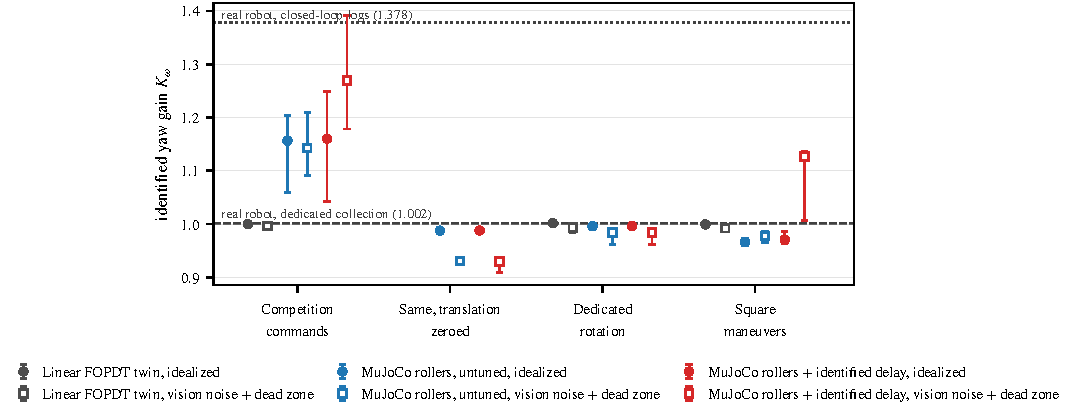
\includegraphics[width=0.74\textwidth]{fig_journal_identifiability.pdf}
  \caption{Yaw gain re-identified from synthetic logs generated by a known plant, by excitation regime. Markers: median over replicates; bars: interquartile range. Horizontal lines: the real robot's estimates from closed-loop competition logs and from the dedicated open-loop collection.}
  \label{fig:ident}
\end{figure*}

% ==============================================================================
% tab_journal_insilico_yaw: generated by `dtssl analysis run journal_tables` (dtssl.analysis.journal_tables).
% Do not edit by hand: re-run the generator. Sources:
%   results/identifiability_insilico_20260907_1552.json
%   results/identifiability_insilico_mujoco-rollers_v2_20260907_2048.json
%   results/identifiability_insilico_mujoco-rollers-delay_v2_20260907_2044.json
%   results/r3_closedloop_omega_fit_20260810_1036.md
%   config/twin_params.json (K_w = 1.0016)
% ==============================================================================
% Needs \usepackage{booktabs,adjustbox}.
\begin{table*}[t]
\centering
\caption{Yaw gain re-identified from synthetic logs generated with a known plant, by excitation regime and generator.}
\label{tab:insilico-yaw}
\small
\begin{adjustbox}{max width=\textwidth}
\begin{tabular}{lcccccc}
\toprule
& \multicolumn{2}{c}{linear FOPDT twin} & \multicolumn{2}{c}{MuJoCo rollers} & \multicolumn{2}{c}{MuJoCo rollers + delay} \\
\cmidrule(lr){2-3} \cmidrule(lr){4-5} \cmidrule(lr){6-7}
regime & idealized & noise + dead zone & idealized & noise + dead zone & idealized & noise + dead zone \\
\midrule
competition commands & 1.000 [1.000, 1.000] & 0.996 [0.996, 0.997] & 1.156 [1.059, 1.204] & 1.143 [1.092, 1.209] & 1.160 [1.043, 1.249] & 1.270 [1.179, 1.391] \\
same, translation zeroed & -- & -- & 0.988 [0.986, 0.989] & 0.931 [0.926, 0.936] & 0.988 [0.987, 0.989] & 0.930 [0.910, 0.937] \\
dedicated rotation & 1.002 [1.002, 1.002] & 0.994 [0.985, 0.995] & 0.996 [0.996, 0.996] & 0.984 [0.962, 0.988] & 0.996 [0.996, 0.996] & 0.984 [0.962, 0.988] \\
square maneuvers & 0.999 [0.999, 1.000] & 0.992 [0.988, 0.995] & 0.967 [0.960, 0.973] & 0.977 [0.966, 0.986] & 0.971 [0.963, 0.987] & 1.127 [1.007, 1.137] \\
designed excitation & 1.001 [1.001, 1.001] & 1.000 [0.999, 1.000] & 1.015 [0.965, 1.057] & 1.065 [1.015, 1.113] & 1.031 [0.981, 1.060] & 0.986 [0.950, 1.021] \\
\bottomrule
\end{tabular}
\end{adjustbox}

\vspace{2pt}
\parbox{\linewidth}{\footnotesize Median [25th, 75th percentile] over replicates (20 for the linear twin, 12 for MuJoCo). Idealized: no measurement noise, dead zone off; noise + dead zone: vision noise of 2 mm and 0.01 rad with the firmware per-wheel dead zone. Designed excitation: R3 for the linear twin, the milder R3-mild inside the traction envelope of the rollers model for MuJoCo. Real robot: 1.378 from closed-loop logs, 1.002 from the dedicated collection.}
\end{table*}


\pending{text of the section.}

%==============================================================================
% 7 RESULTS II: CROSS-COUPLING
% Executado em 14/10/2026 (CHANGELOG 2026-10-14 12:11): coupled_mimo_check (primaria,
% atrasos por par, bootstrap, harness) + controles C- (fopdt) e C+ (mujoco-rollers-delay).
% Tabela gerada: tables/tab_journal_coupling (dtssl analysis run journal_tables --kw
% tables=coupling). Fontes: results/coupled_mimo_check_20261014_1211.{md,json},
% results/coupled_mimo_check_control-fopdt_20261014_1211.json,
% results/coupled_mimo_check_control-mujoco-rollers-delay_20261014_1216.json;
% pre-registro docs/PREREGISTRO_MIMO_CHECK_20260923.md (as frases do §8 estao usadas
% no paragrafo M1). Rascunho de 14/10 escrito a partir dos artefatos; revisar a voz.
%==============================================================================
\section{Results II: cross-coupling between channels}
\label{sec:res-coupling}

% ==============================================================================
% tab_journal_coupling: generated by `dtssl analysis run journal_tables` (dtssl.analysis.journal_tables).
% Do not edit by hand: re-run the generator. Sources:
%   results/coupled_mimo_check_20261014_1211.json
%   results/coupled_mimo_check_control-fopdt_20261014_1211.json
%   results/coupled_mimo_check_control-mujoco-rollers-delay_20261014_1216.json
%   results/CHANGELOG.md 2026-10-14 12:11
%   docs/PREREGISTRO_MIMO_CHECK_20260923.md
% ==============================================================================
% Needs \usepackage{booktabs,adjustbox}.
\begin{table*}[t]
\centering
\caption{Cross-coupling check on the competition logs: per-DOF against coupled first-order structure, scored on the frozen hold-out, with the pre-registered verdicts.}
\label{tab:coupling}
\small
\begin{adjustbox}{max width=\textwidth}
\begin{tabular}{lccc}
\toprule
& $v_x$ & $v_y$ & $\omega$ \\
\midrule
pooled hold-out fit (\%): promoted plant & 75.3 & 79.7 & 40.1 \\
\quad diagonal re-fit & 75.5 & 79.9 & 48.8 \\
\quad coupled & 76.5 & 80.1 & 48.9 \\
fit gain, coupled vs. diagonal (p.p.) [95\% CI] & +0.95 [+0.62, +1.07] & +0.23 [+0.02, +0.30] & +0.13 [-0.05, +0.15] \\
cross / direct RMS ratio [95\% CI] & 0.058 [0.046, 0.076] & 0.039 [0.019, 0.059] & 0.048 [0.026, 0.074] \\
direct gain, diagonal / coupled & 1.100 / 1.105 & 1.067 / 1.067 & 1.419 / 1.414 \\
largest cross gain (source) & -0.045 (from $v_y$) & -0.065 (from $\omega$) & -0.047 (from $v_y$) \\
M1 ($\geq 3$ p.p. and ratio $\geq 0.10$): coupling matters & no & no & no \\
\midrule
\multicolumn{4}{l}{free-run $\epos$ at $\hRef$, per-window median (m): promoted 0.0388, diagonal 0.0390, coupled 0.0381} \\
\multicolumn{4}{l}{M3 (gate 8/10, $p<0.05$, $r_b \geq 0.5$): coupled beats diagonal 6/10, $p = 0.46$, $r_b = +0.05$: no} \\
\multicolumn{4}{l}{M2 (half of the excess over 1.0016 open loop): direct yaw gain 1.419 $\rightarrow$ 1.414 with the translational inputs, 1\% removed: falsified} \\
\multicolumn{4}{l}{C$-$ (promoted twin as generator): $G_{\omega\omega}$ 0.9997 / 0.9997 against 1.0017; no spurious coupling: passed} \\
\multicolumn{4}{l}{C$+$ (MuJoCo route b with delay as generator): inflation +7.2\%, below the 10\% premise: not testable} \\
\multicolumn{4}{l}{C$+$, post hoc: $\omega$ from $v_y$ 0.216 of the direct term; $G_{\omega\omega}$ 1.068 $\rightarrow$ 1.075} \\
\bottomrule
\end{tabular}
\end{adjustbox}

\vspace{2pt}
\parbox{\linewidth}{\footnotesize Same estimator (separable least squares on the simulation error), same 36 training events and the same 10 frozen hold-out events for both arms; delays fixed at the promoted plant's 5/4/6 samples. Bootstrap over training events (200 replicates, percentile intervals). The free-run rows use the paper's harness (re-anchored windows, translational bin). The in-silico controls run the same pipeline on noise-free logs generated from the recorded commands.}
\end{table*}


The per-DOF structure of Section~\ref{sec:models} treats $v_x$, $v_y$ and $\omega$ as three independent first-order plants. The natural objection is that it ignores coupling between channels, and the in-silico result of Section~\ref{sec:res-ident} gives that objection a concrete form: in a physical generator, translation induces yaw that is correlated with the yaw command, and the closed-loop yaw gain is inflated by it. We therefore pre-registered three questions before any number was computed on the robot data. M1 (primary): do cross-command terms, added to the same first-order model and fitted with the same estimator on the same 36 training events, improve what the model reproduces on the frozen hold-out? M2 (mechanism): does giving the yaw channel the translational commands as inputs pull the direct yaw gain estimated from the closed-loop logs towards the value of the dedicated open-loop collection? M3 (use): does the coupled model lower the free-run position error of the harness of Section~\ref{sec:protocol}, on the same windows as every other number of this paper? The decision rules, the two in-silico controls and both possible wordings of the outcome were fixed in the pre-registration, and the run followed it without change.

\paragraph{Design.} Both arms share the model $y_i[k] = A_i\,y_i[k-1] + \sum_j B_{ij}\,u_j[k-1-M_{ij}]$ on the 60~Hz grid, the plant alignment of the harness and the delays of the promoted plant (5, 4 and 6 samples for $v_x$, $v_y$ and $\omega$). The diagonal arm sets $B_{ij} = 0$ for $i \neq j$ and is the per-DOF structure re-estimated on the training events; the coupled arm fits the full $3 \times 3$ matrix $B$ with one pole per output. The estimator is the same for both: for a fixed pole the simulated output is linear in the row of $B$, so each row is a separable least-squares problem on the simulation error, the error that the protocol scores, with the pole found by a one-dimensional search. The promoted plant of the paper is scored alongside as the anchor of the published numbers. Coupling is read on two scales at once, the gain in pooled hold-out fit and the ratio between the RMS of the cross terms and the RMS of the direct term, because a cross gain is only interpretable when the term it multiplies contributes to the response. A bootstrap over training events gives the intervals of Table~\ref{tab:coupling}.

\paragraph{M1: coupling does not matter in the envelope of these logs.} A coupled first-order model with cross-command terms, fitted with the same estimator on the same training events, changes the pooled hold-out fit by less than 1~p.p.\ on every DOF, and its cross terms stay below 6\,\% of the direct term's RMS (Table~\ref{tab:coupling}); the largest cross gain, from $v_y$ into $v_x$, is $-0.045$ against a direct gain of 1.105. Neither threshold of the pre-registered rule (3~p.p.\ and a ratio of 0.10 on the same DOF) is reached, and the bootstrap intervals of the fit gains exclude 3~p.p.\ on all three channels. Searching the delay of every input-output pair exhaustively between 0 and 10 samples, the secondary analysis of the pre-registration, moves the pooled fits by at most 1.6~p.p.\ and leaves the verdict unchanged. Within the envelope of these logs the decoupled structure loses nothing measurable; aggressive mixed motion, which the competition logs do not contain, is where a coupled model would have to be tested.

\paragraph{M2: the closed-loop yaw bias is not a linear function of the translational commands.} The premise of the mechanism test is reproduced. Re-estimated on the 36 closed-loop events, the direct yaw gain of the diagonal arm is 1.419 (95\,\% interval 1.360 to 1.517), 41.7\,\% above the 1.0016 of the dedicated open-loop collection and in line with the 1.378 that the prediction-error estimator of Section~\ref{sec:res-ident} gives on the same logs, the correlation bias that direct identification in closed loop is known to carry~\cite{forssell1999closedloop}. Giving the yaw channel the translational commands as inputs leaves the gain at 1.414, which removes 1\,\% of the excess; the rule required half. Restricting the training set to the 13 events of the game label, or searching the delays per pair, does not change the outcome. The hypothesis is falsified in the form it was stated: whatever produces the excess gain is not captured by a term linear in the commanded $v_x$ and $v_y$. The in-silico mechanism of Section~\ref{sec:res-ident} is not thereby refuted, because the pre-registration already stated that a sign-symmetric effect, proportional to $|v|$ for instance, would appear as unexplained variance rather than as a cross gain; the positive control below sharpens that reading.

\paragraph{M3: no gain in use.} In the free-run harness the coupled plant beats the diagonal re-fit in 6 of the 10 hold-out events (one-sided Wilcoxon $p = 0.46$, rank-biserial $+0.05$), short of the gate of 8 of 10 that every other per-event comparison of this paper uses; the per-window medians at $\hRef$ are 0.0388, 0.0390 and 0.0381~m for the promoted, diagonal and coupled plants, within 1~mm of each other. Neither re-fitted arm beats the promoted plant either (5 and 4 of 10 events). The sanity check of the harness reproduces the per-event median of the promoted plant, 0.0421~m, exactly.

\paragraph{Controls.} The negative control runs the same pipeline on noise-free logs generated from the recorded commands by the promoted twin, which has no coupling: both arms recover the yaw gain of the generator to within 0.2\,\% and every cross ratio stays below $10^{-3}$, so the pipeline does not invent coupling and the verdicts on the robot data are interpretable. The positive control replaces the generator by the untuned MuJoCo route~b with the identified delay, the physical generator whose closed-loop yaw inflation Section~\ref{sec:res-ident} reports. With this estimator and all 36 training events the inflation it produces is 7.2\,\% (8.3\,\% on the game label), below the 10\,\% premise fixed in the pre-registration, so the positive control is formally not testable and we report it as such. Its direction is nevertheless informative, and we read it post hoc: the coupled arm does detect the physical coupling, with a cross term from $v_y$ into $\omega$ worth 0.216 of the direct term, the only ratio above 0.10 in the whole study, and still does not lower the direct yaw gain (1.068 to 1.075). A linear cross-command term does not absorb the excess of the direct gain even in a generator where translation-induced yaw is known to exist, and that is the reading we give to the falsification of M2 on the robot.

\paragraph{What the check settles.} The decoupled plant is not a simplification that the data would overturn: at the fidelity the harness measures, the three channels of this robot can be identified separately from operational logs, and the one channel that closed-loop logs identify badly, yaw, is not repaired by coupling but by the short dedicated collection of Section~\ref{sec:res-ident}. The check also bounds what a coupled extension could bring, less than 1~p.p.\ of hold-out fit and no measurable change in free-run error, until data with aggressive mixed motion exist.

%==============================================================================
% 8 RESULTS III: FIDELITY AGAINST EVERY BASELINE
% Plano: o modelo contra cinematica ideal, rSim (stock, e com atraso casado), MuJoCo
% rota a (embedding = gemeo) e rota b (sem sintonia, com atraso), grSim e ER-Force
% (teleporte cru, +atraso, pre-rolagem; tres sessoes: 10/09, 18/09, 20/09);
% repetibilidade entre sessoes (as tres sessoes lado a lado na tabela); condicao inicial (modelo com estados zerados 0.1137, pre-rolado 0.0406);
% atribuicao de Shapley; v0 causal; LOO; controle negativo bayesiano; heading.
% Baseline sintonizada (C3 ou rSim): so se a orientadora aprovar (WP3).
% Fontes: tab_journal_baselines, tab_journal_robustness, fig_journal_league_sims
% (geradas); CHANGELOG 2026-09-07 15:15 (C2a), 2026-09-10 02:11 (C2b),
% 2026-09-18 13:26 (C2b2 sessao 1, entrada do lote 1), 2026-09-20 11:43 (C2b2 sessao 2).
%==============================================================================
\section{Results III: fidelity against physics and league simulators}
\label{sec:res-fidelity}

% ==============================================================================
% tab_journal_baselines: generated by `dtssl analysis run journal_tables` (dtssl.analysis.journal_tables).
% Do not edit by hand: re-run the generator. Sources:
%   results/epos_eang_three_models_20260810_1022.md
%   results/negcontrol_perevent_20260810_1035.md
%   results/eval_rsim_delay_ablation_20260809_2154.md
%   results/backends_holdout_20260907_1515.md
%   results/backends_holdout_20260907_1515.csv
%   results/protocol_holdout_20260910_0211.json
%   results/protocol_holdout_20260918_1326.json
%   results/protocol_holdout_20260920_1143.json
% ==============================================================================
% Needs \usepackage{booktabs,adjustbox}.
\begin{table*}[t]
\centering
\caption{Every baseline scored on the same windows and metric as the identified model.}
\label{tab:baselines}
\small
\begin{adjustbox}{max width=\textwidth}
\begin{tabular}{llcccc}
\toprule
plant & session & $e_{\mathrm{pos}}$ per window (m) & $e_{\mathrm{pos}}$ per event (m) & model wins & $p$ \\
\midrule
Identified model & in process & 0.0388 & 0.0421 & -- & -- \\
Model, states zeroed at $t_0$ & in process & 0.1137 & -- & -- & -- \\
Model, pre-rolled & in process & 0.0406 & -- & -- & -- \\
\midrule
Ideal kinematics & in process & 0.1005 & 0.1177 & 10/10 & $9.8\times10^{-4}$ \\
rSim, stock parameters & in process & 0.1293 & -- & -- & -- \\
rSim, stock + matched delay & in process & 0.1822 & -- & -- & -- \\
MuJoCo, velocity-driven (route a) & in process & 0.0388 & 0.0421 & 7/10 & $0.22$ \\
MuJoCo rollers, untuned (route b) & in process & 0.0729 & 0.0791 & 10/10 & $9.8\times10^{-4}$ \\
MuJoCo rollers + delay & in process & 0.0477 & 0.0487 & 9/10 & $9.8\times10^{-3}$ \\
\midrule
grSim, teleport (rest) & 09-10 / 09-18 / 09-20 & 0.2389 / 0.2421 / 0.2329 & 0.2341 / 0.2398 / 0.2299 & 10/10 / 10/10 / 10/10 & $9.8\times10^{-4}$ \\
grSim + delay & 09-10 & 0.2335 & 0.2345 & 10/10 & $9.8\times10^{-4}$ \\
grSim, pre-rolled & 09-18 / 09-20 & 0.0996 / 0.0809 & 0.1106 / 0.0975 & 10/10 / 10/10 & $9.8\times10^{-4}$ \\
ER-Force, teleport & 09-10 / 09-18 / 09-20 & 0.0881 / 0.0856 / 0.0874 & 0.1006 / 0.1023 / 0.0995 & 10/10 / 10/10 / 10/10 & $9.8\times10^{-4}$ \\
ER-Force + delay & 09-10 & 0.0555 & 0.0555 & 9/10 & $2.0\times10^{-3}$ \\
ER-Force, pre-rolled & 09-18 / 09-20 & 0.0934 / 0.0940 & 0.1114 / 0.1114 & 10/10 / 10/10 & $9.8\times10^{-4}$ \\
\bottomrule
\end{tabular}
\end{adjustbox}

\vspace{2pt}
\parbox{\linewidth}{\footnotesize Median position error at $h_{\mathrm{ref}} = 0.4$ s on the translation-dominated hold-out windows: over windows, and the median of the ten per-event medians; model wins and one-sided paired Wilcoxon $p$ per event (model $<$ plant; $p$ shown once where equal in every session). Sessions are dates of the real-time protocol replays (2026). Dashes: not computed per event in the artefact.}
\end{table*}


\begin{figure*}[t]
  \centering
  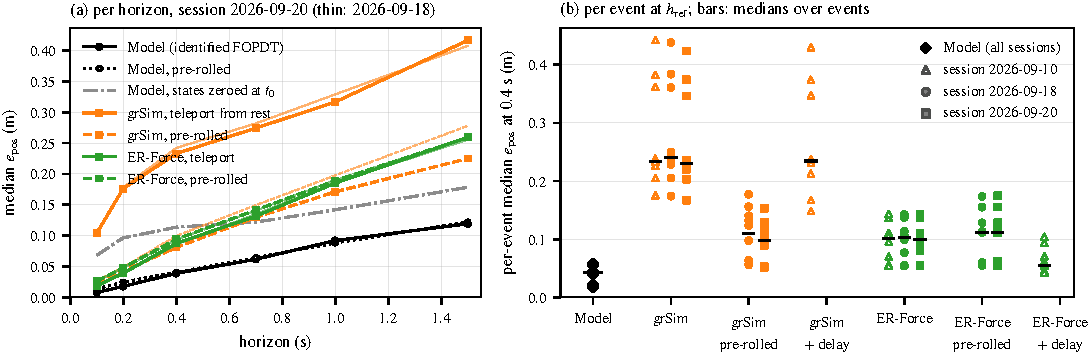
\includegraphics[width=\textwidth]{fig_journal_league_sims.pdf}
  \caption{League simulators replayed through the simulation protocol on the hold-out windows. (a) Median position error per horizon; the pre-roll lets each simulator reach the anchor with its own dynamics. (b) Per-event medians at the reference horizon in every session.}
  \label{fig:league}
\end{figure*}

% ==============================================================================
% tab_journal_robustness: generated by `dtssl analysis run journal_tables` (dtssl.analysis.journal_tables).
% Do not edit by hand: re-run the generator. Sources:
%   results/ablation_orderfree_20260810_1021.md
%   results/causal_ic_check_20260810_1102.md
%   results/gate_window_vs_event_20260810_1743.md
%   results/negcontrol_perevent_20260810_1035.md
%   results/eval_rsim_delay_ablation_20260809_2154.md
%   results/loo_translational_20260810_1743.md
% ==============================================================================
% Needs \usepackage{booktabs,adjustbox}.
\begin{table*}[t]
\centering
\caption{Robustness of the fidelity result.}
\label{tab:robustness}
\small
\begin{adjustbox}{max width=\textwidth}
\begin{tabular}{lp{0.62\linewidth}}
\toprule
check & result (position error at $h_{\mathrm{ref}} = 0.4$ s unless stated) \\
\midrule
Order-free attribution of the gain over ideal kinematics (0.0617 m) & $\tau$ 55\%, $T_d$ 43\%, $K$ 2\% \\
Measured initial velocity & constant-velocity extrapolation 0.1600 m; model from rest 0.1137 m; model with measured velocity 0.0388 m \\
Strictly causal initial velocity & 0.0468 m (central 0.0388 m); per-event gap +0.0706 m, 10/10, $p = 9.8\times10^{-4}$ \\
Unit of analysis & windows ($n=49$): gap +0.0541 m, $p = 1.2\times10^{-8}$, $r_{rb} = 0.633$; events ($n=10$): gap +0.0689 m, $p = 9.8\times10^{-4}$, $r_{rb} = 1.000$ \\
Negative control (9-parameter Bayesian calibration) & per-event gap +0.0038 m, 7/10, $p = 0.042$, $r_{rb} = 0.40$ \\
rSim with the model's transport delay & 0.1293 $\rightarrow$ 0.1822 m (gap widens) \\
Leave-one-event-out fit & $v_x$ $84.3\pm2.0$\% (4 folds); $v_y$ $82.8\pm2.7$\% (13 folds) \\
\bottomrule
\end{tabular}
\end{adjustbox}
\end{table*}


\pending{text of the section.}

%==============================================================================
% 9 RESULTS IV: CLOSED-LOOP PLAUSIBILITY
% Plano: a estrategia real jogando contra o gemeo (sessao B3, 220 s, 6 robos);
% round trip recorder -> harness ao nivel do mm; C4: 2/5 contra o pool
% (pre-registrado), 5/5 contra shoot_to_goal (pos-hoc, declarado); o regime de yaw
% diluido reaparece; rastreamento 0.865 vs 0.944 (descritivo).
% Fontes: tab_journal_closed_loop, fig_journal_closed_loop (geradas);
% results/session_report_sessao_01_20260907_2059.md; CHANGELOG 2026-09-07 20:59 e 21:37.
%==============================================================================
\section{Results IV: closed-loop plausibility}
\label{sec:res-closed}

\begin{figure*}[t]
  \centering
  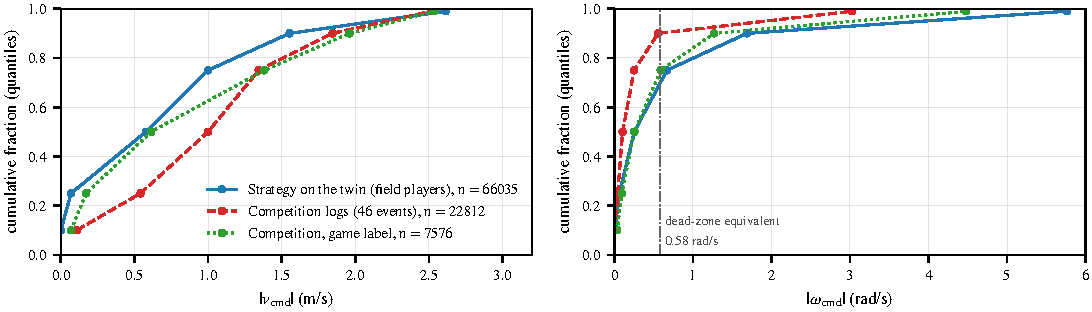
\includegraphics[width=\textwidth]{fig_journal_closed_loop.pdf}
  \caption{Commands of the team's strategy playing against the twin, against the competition logs: cumulative distributions of the commanded speed and yaw rate. Vertical line: body yaw rate equivalent to the firmware per-wheel dead zone.}
  \label{fig:closed}
\end{figure*}

% ==============================================================================
% tab_journal_closed_loop: generated by `dtssl analysis run journal_tables` (dtssl.analysis.journal_tables).
% Do not edit by hand: re-run the generator. Sources:
%   results/closed_loop_stats_20260907_2137.json
%   results/CHANGELOG.md 2026-09-07 21:37 (post hoc game-label reading)
% ==============================================================================
% Needs \usepackage{booktabs,adjustbox}.
\begin{table*}[t]
\centering
\caption{Closed-loop plausibility: what the strategy commands when it plays against the twin.}
\label{tab:closed-loop}
\small
\begin{adjustbox}{max width=\textwidth}
\begin{tabular}{lccc}
\toprule
& strategy on the twin (field players) & competition pool (46 events) & competition, game label \\
\midrule
samples at 60 Hz & 66035 & 22812 & 7576 \\
$|v_{\mathrm{cmd}}|$ median (m/s) & 0.578 & 1.000 & 0.614 \\
$|v_{\mathrm{cmd}}|$ 90th percentile (m/s) & 1.554 & 1.846 & 1.962 \\
$|\omega_{\mathrm{cmd}}|$ median (rad/s) & 0.251 & 0.104 & 0.254 \\
$|\omega_{\mathrm{cmd}}|$ 90th percentile (rad/s) & 1.687 & 0.556 & 1.269 \\
$|\omega_{\mathrm{cmd}}| < 0.58$ rad/s (\%) & 71.8 & 90.5 & 74.5 \\
dead zone alters / zeroes the command (\%) & 27.3 / 7.8 & 16.0 / 2.6 & 31.7 / 6.7 \\
idle (\%) & 12.6 & 1.4 & 3.6 \\
$|v_{\mathrm{cmd}}| > 2.9$ m/s (\%) & 0.31 & 0.01 & 0.01 \\
\midrule
$W_1$ distance of $|v|$ / $|\omega|$ to the session & -- & 0.326 / 0.387 & 0.179 / 0.127 \\
pre-registered plausibility criteria met & -- & 2/5 & 5/5 (post hoc) \\
\bottomrule
\end{tabular}
\end{adjustbox}

\vspace{2pt}
\parbox{\linewidth}{\footnotesize Commands of the team's real strategy closing the loop on the twin (recorded session, goalkeeper excluded) against the competition logs on the same 60 Hz grid. The pre-registered reference was the whole pool; 28 of its 46 events are scripted maneuvers, so the comparison with the game label is reported as post hoc.}
\end{table*}


\pending{text of the section.}

%==============================================================================
% 10 DISCUSSION
% Plano: o que o modelo compra (tau e Td, condicionados a velocidade medida);
% identificabilidade como propriedade do dado; quando um gemeo fisico e necessario
% (rota b + atraso chega perto, sem sintonia); regra de triagem na pratica;
% generalizacao do protocolo a outros gemeos (sem prometer RL nem Isaac Sim).
%==============================================================================
\section{Discussion}
\label{sec:discussion}

\pending{what the model buys; identifiability as a property of the data; when a physics twin is needed; the screening rule in practice.}

%==============================================================================
% 11 LIMITATIONS AND THREATS TO VALIDITY
% Plano: as sete limitacoes do SBR (amostra de yaw pequena e de uma sessao; um robo
% e um contexto; contraste nao single-factor; estimadores closed-loop-aware nao
% tentados; Ljung-Box; constantes cinematicas; rSim sem sintonia) + as do camera-ready
% (desacoplamento, sem saturacao/aceleracao/zona morta, slip so pelos parametros,
% envelope dos dados) + as novas (instrumento em tempo real; tau0 do grSim; ER-Force
% sem omega no teleporte; repetibilidade da pre-rolagem do grSim entre sessoes;
% pre-registros com referencia errada mantidos; hold-out 99.6 % translacional).
% Observacao: a versao integra de 9 paragrafos das limitacoes nao existe mais em
% disco nem no git (latex/ so entrou no git em 02/09); reescrever a partir das fontes
% (backlog JINT item A, CHANGELOG, artefatos).
%==============================================================================
\section{Limitations and threats to validity}
\label{sec:limitations}

\pending{data and identification; evaluation and scope; instrument; declared deviations.}

%==============================================================================
% 12 CONCLUSION + DATA AND CODE AVAILABILITY + CRediT + DECLARATIONS
% Availability: repositorio publico + DOI (WP5, D3 congelado); logs de competicao,
% coleta dedicada e sessao B3 via DVC; um `dtssl analysis run <nome>` por numero.
%==============================================================================
\section{Conclusion}
\label{sec:conclusion}

\pending{conclusion.}

\section*{Data and code availability}
\pending{repository, DOI, datasets and the command that reproduces each number.}

\section*{CRediT authorship contribution statement}
\pending{CRediT roles (decide authorship with the advisor).}

\section*{Declaration of competing interest}
\pending{declaration.}

\section*{Declaration of generative AI and AI-assisted technologies in the writing process}
\pending{declaration required by Elsevier: which tools were used, for what, and that the authors reviewed and take responsibility for the content.}

\section*{Acknowledgements}
\pending{funding and acknowledgements.}


\bibliographystyle{elsarticle-num}
\bibliography{refs/references,refs/own}

\end{document}
